\begin{theo}[Elektrische ladingen]{Elektrische ladingen}
    \begin{itemize}
        \item tegengestelde ladingen trekken elkaar aan en gelijke ladingen stoten elkaar af
        \item gekwantiseerde grootheid, geen fracties
    \end{itemize}
\end{theo}

\begin{lem}[Behoud van totale lading]{Behoud van totale lading}
    Bij een geïsoleerd systeem blijft de totale aantal lading gelijk, er is enkel \textbf{transfert} van lading
\end{lem}

\begin{app}[Elektrische lading in het atoom – isolator $ \leftrightarrow $ geleider]{Elektrische lading in het atoom  isolator geleider}

    \begin{itemize}
        \item \textbf{Geleider:} \underline{sommige} elektronen zijn ongebonden en kunnen vrij bewegen
        \item \textbf{Isolator:} \underline{alle} elektronen zijn gebonden en onbeweegelijk
        \item \textbf{Halfgeleider:} ergens tussenin
    \end{itemize}

\end{app}

\begin{theo}[Coulombkracht]{Coulombkracht}

    Coulomb concludeerde dat de kracht die een klein geladen voorwerp uitoefent op een tweede evenredig is met het product van de magnitude van de lading op de ene, $ q_1 $, maal de magnitude van de lading op de andere, $ q_2 $, en omgekeerd evenredig met het kwadraat van de afstand $ r $ tussen beide. In formulevorm wordt dit:
    
    \begin{equation*}
        \hspace{3cm} \Vec{F}_{e} = k_e\dfrac{q_1q_2}{r^2}\hat{r} \quad \quad (\text{met } k_e = \dfrac{1} {4\pi\epsilon_0})
    \end{equation*}
    
    % \noindent In de bovenstaande formule komen wat nieuwe letters aan bod, namelijk $ k_e $ en $ \epsilon_0 $. Het eerste kent men als de \textbf{Coulomb constante}, het tweede als de \textbf{permitiviteit} van het vacuum. \\
    
    % \noindent Bij meerdere coulombkrachten kunnen we het principe van superpositie toepassen:
    %     \begin{itemize}
    %         \item \textbf{Discreet:} $ \Vec{F}_{e^*} = k_e q^* \sum_i \dfrac{q_i}{r_i^2}\hat{r}_i$
    %         \item \textbf{Continu:} $ \Vec{F}_{e^*} = k_e q^* \int \dfrac{1}{r^2}\hat{r} dq$
    %     \end{itemize}
    % \noindent We zien ook een duidelijk verband met de zwaartekracht: vervang het concept van lading door het concept van massa en je komt de gravitatiekracht uit. Hetzelfde geldt voor het latere concept van een elektrisch veld met het gravitatieveld. \\

    \noindent \textbf{Opmerking:} de lading bij de coulombkracht is telkens de absolute waarde, omdat de grootte van een vector niet negatief mag zijn. De richting wordt dus bepaald door $\hat{r}$.
\end{theo}

\begin{theo}[Elektrisch veld]{Elektrisch veld}

    De elektrische veld vector $ \Vec{E} $ in een punt in de ruimte is gelijk aan de elektrische kracht $ \Vec{F_e} $ die op een \textbf{positieve} testlading werkt, gedeeld door de testlading. In formulevorm:
    
    \begin{equation*}
        \Vec{E} = \dfrac{\Vec{F_e}}{q} =  k_e\dfrac{q}{r^2}\hat{r}
    \end{equation*}
    
    % \noindent We vinden nu dus ook de volgende interessante formules als we spreken over een punt tegenover een puntlading:
    
    % \begin{align}
    %     \hspace{3.5cm}\Vec{F_e} &= \Vec{E}q \\
    %     \Vec{E} &= k_e\dfrac{q}{r^2}\hat{r} \quad \quad (\Vec{F}_{e} = k_e\dfrac{q_1q_2}{r^2}\hat{r})
    % \end{align}
    
    % \noindent Formules (1) en (2) kunnen we ook gebruiken als we spreken over meerdere puntladingen door opnieuw het principe van superpositie te gebruiken.

\end{theo}

\newpage

\begin{app}[Beweging van een lading in een uniform elektrisch veld]{Beweging van een lading in een uniform elektrisch veld}
    \begin{minipage}{.7 \textwidth}
        \vspace{-0.15cm}
        We vinden door de tweede wet van Newton toe te passen:
        \begin{align*}
            \Vec{F}_{net} &= \sum \Vec{F} = m\Vec{a} \\
                          &= \Vec{F_e} = q\Vec{E} = m\Vec{a}
        \end{align*}
        \noindent Hieruit volgt dus de vectoriële formule voor de versnelling veroorzaakt door een uniform elektrisch veld, namelijk:
        \begin{equation*}
            \Vec{a} = \dfrac{q}{m}\Vec{E}
        \end{equation*}
        Sinds dat de massa, het elektrisch veld en de lading constant is, blijft dus de versnelling \textbf{ook constant}! We kunnen dus de veelbesproken identiteiten hiervoor gebruiken.
    \end{minipage} 
    \begin{minipage}{.30\textwidth}
        \vspace{-0.3cm}
        \centering
        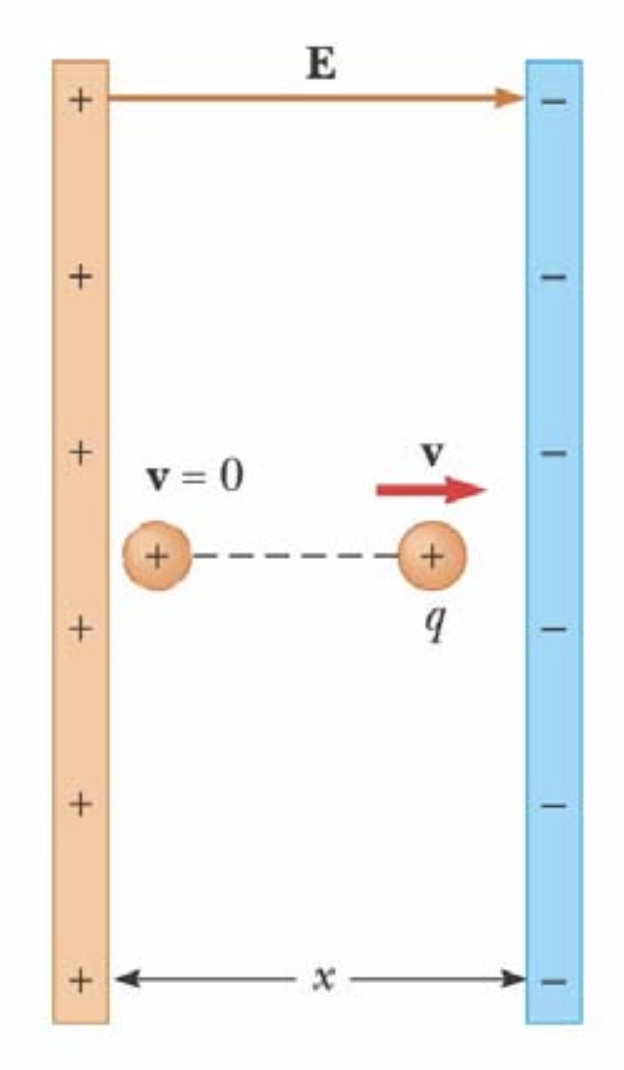
\includegraphics[scale = 0.3]{Images/Elektriciteit/UniformE.png}
    \end{minipage}

\end{app}

\begin{pro}[Geleiders in elektrostatisch evenwicht]{Geleiders in elektrostatisch evenwicht}
    \begin{itemize}
        \item Het elektrisch veld in een geleider is nul (bij elektrostatisch evenwicht mag er geen \textbf{netto} ladingsbeweging zijn)
        \item De lading van een geïsoleerde geleider bevindt zich aan het oppervlak
        \item Het elektrisch veld net buiten de geleider is loodrecht op het oppervlak en $|E| = \tfrac{\sigma}{\epsilon_0}$
        \item Oppervlakteladingsdichtheid $\sigma$ is het grootst bij de grootste oppervlaktekromming
    \end{itemize}
\end{pro}

\begin{app}[Elektrisch veld berekeningen voor continue ladingsverdelingen]{Elektrisch veld berekeningen voor continue ladingsverdelingen}

    We kunnen bij continue ladingen een infinitesimaal gebied bekijken, hier dus een infinitesimale lading en krijgen we de volgende formule:
    
    \begin{equation}
        d\Vec{E} = k_e \dfrac{dq}{r^2}\hat{r}
    \end{equation}
    
    \noindent We willen nu het totale veld bereken door te sommen over al deze infinitesimalen:
    
    \begin{equation}
        \Vec{E} = \int d\Vec{E}
    \end{equation}
    
    \noindent Als we nu een \textbf{uniforme ladingsdichtheid} definiëren, dan kunnen we meeste berekeningen oplossen omtrent continue ladings verdelingen. We definiëren:

    % \begin{equation*}
    %     dq = \rho dV = \sigma dA = \lambda dL
    % \end{equation*}
    
    \begin{itemize}
        \item \textbf{Volume-ladingsverdeling:} $ \rho = \dfrac{dq}{dV} $
        \item \textbf{Oppervlakte-ladingsverdeling:} $ \sigma = \dfrac{dq}{dA} $
        \item \textbf{Lineaire-ladingsverdeling:} $ \lambda = \dfrac{dq}{dL} $
    \end{itemize}

    \vspace{-0.3cm}
    
\end{app}

\newpage

\begin{theo}[Elektrische dipool en het dipoolmoment]{Elektrische dipool en het dipoolmoment}

    Wanneer er 2 gelijke ladingen zijn met tegengesteld teken, dus: $ +q \ en \ -q $, en ze gescheiden zijn door een lengte $ \ell $, dan kunnen we spreken over een \textbf{elektrisch dipool}. \\
    \begin{center}
       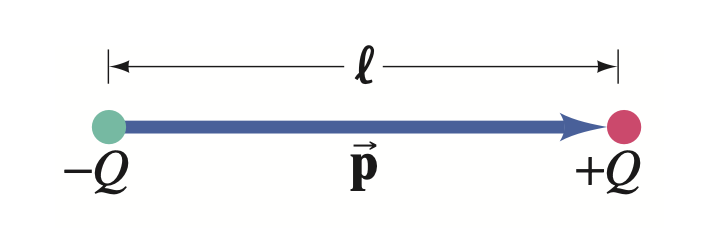
\includegraphics[scale = 0.4]{Images/Elektriciteit/Dipool.png} 
    \end{center}
    Het elektrisch dipoolmoment $ \vec{p} $ is een maat van polariteit van een binding en kan als volgt vectorieel weergegeven worden: 
    
    \begin{equation*}
        \Vec{p} = q\Vec{\ell}
    \end{equation*}
\end{theo}

\begin{app}[Dipool in een uniform veld]{Dipool in een uniform veld}
    
    \begin{minipage}{.48\textwidth}
        \begin{itemize}
            \item \textbf{Totale kracht:}
                \begin{equation*}
                    \vspace{0.25cm}
                    \Vec{F} = \Vec{F}_++\Vec{F}_- = q\Vec{E} - q\Vec{E} = 0
                \end{equation*}
            \item \textbf{Krachtmoment rond middelpunt:}
                \begin{align*}
                     \tau &= qE\dfrac{\ell}{2}\sin(\theta) - (-qE\dfrac{\ell}{2}\sin(\theta)) \\
                     &= qE\dfrac{\ell}{2}\sin(\theta) + qE\dfrac{\ell}{2}\sin(\theta)  \\
                     &= pE\sin(\theta)  \\
                     \Vec{\tau} &= \Vec{p} \times \Vec{E}
                \end{align*}
            \item \textbf{Arbeid:}
        \end{itemize}
    \end{minipage} 
    \begin{minipage}{.48\textwidth}
        \centering
        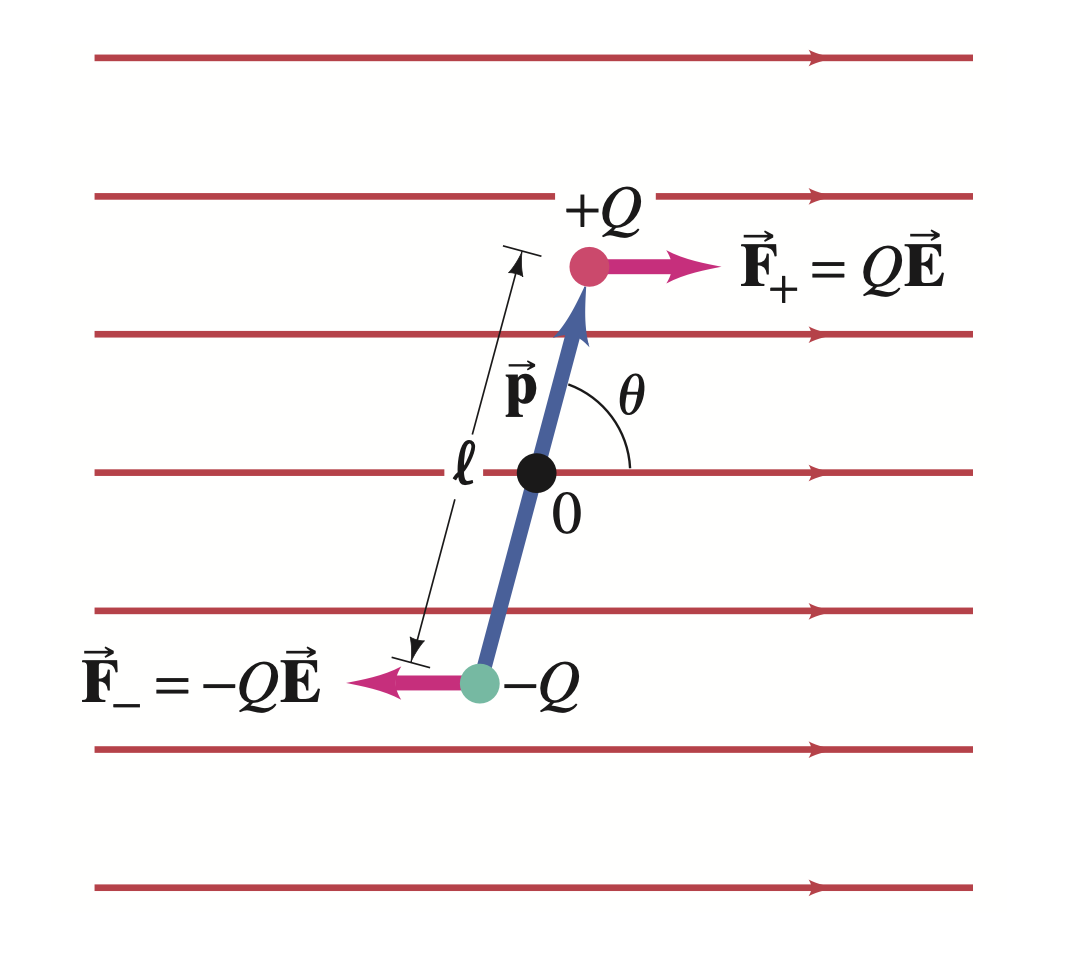
\includegraphics[scale = 0.35]{Images/Elektriciteit/UniformDipool.png}
    \end{minipage}
    
    \begin{minipage}{.5\textwidth}
            \begin{align*}
                \hspace{1.1cm}
                W &= \int_{\theta_1}^{\theta_2} \tau d\theta \\ 
                  &= \textbf{-}pE\int_{\theta_1}^{\theta_2} \sin(\theta) d\theta \quad \quad (\text{$d\theta$ is negatief dus, - voor positieve $W$}) \\
                  &= pE(\cos(\theta_{2})-\cos(\theta_{1})) \\
                  &= -\Delta U \\ 
                U &= -\Vec{p} \cdot \Vec{E} \quad \quad (intertiaalstelsel: \theta_1 = \dfrac{\pi}{2}) \\\\
           \end{align*}
    \end{minipage} 
    \begin{minipage}{.5\textwidth}
    \end{minipage}
    \vspace{-1cm}
\end{app}